\documentclass[border=5pt]{standalone}
\usepackage{tikz}
\usetikzlibrary{calc}
\usepackage{amsmath}
\begin{document}
    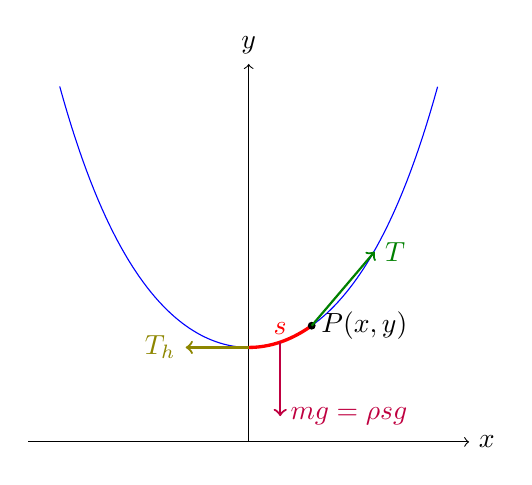
\begin{tikzpicture}[scale=0.8]
        % Draw the catenary curve
        \draw[blue, domain=-3:3, samples=100] plot (\x, {1.5*cosh(\x/1.5)});

        % Draw the coordinate axes
        \draw[->] (-3.5,0) -- (3.5,0) node[right] {$x$};
        \draw[->] (0,0) -- (0,6) node[above] {$y$};

        % Draw the arc length s
        \draw[red, very thick, domain=0:1, samples=100] plot (\x, {1.5*cosh(\x/1.5)});
        \node[red] at (0.5,1.8) {$s$};

        % Mark a point P(x,y)
        \node[circle, fill, inner sep=1pt] (P) at (1,1.8452) {};
        \node[right] at (1,1.8452) {$P(x,y)$};

        \draw[->,thick,olive] (0,1.5) -- (-1,1.5) node[left] {$T_h$};
        \draw[->,thick,green!50!black] (1,1.8452) -- (2,3.0204) node[right] {$T$};
        \draw[->,thick,purple] (0.5,1.5841) -- (0.5,0.41) node[right] {$mg=\rho sg$};



    \end{tikzpicture}
\end{document}
